\section{ICA by maximizing nongaussianity}

\mode<presentation>{
\begin{frame} 
    \begin{center} \huge
        \secname
    \end{center}
    \begin{center}
    Maximizing nongaussianity leads to independent sources
    \end{center}
\end{frame}
}

\begin{frame}{Maximizing nongaussianity}

\begin{block}{Intuition from the Central Limit Theorem}
\emph{The distribution of the sum of independent random variables is ``more Gaussian'' than the original distributions of the random variables.}\\\vspace{2mm}
Searching for the direction of maximum deviation from a Gaussian distribution may recover the original sources.
\end{block}

\begin{center}
    \includegraphics<2>[width=0.8\textwidth]{./img/clt_uniform_0}
    \includegraphics<3>[width=0.8\textwidth]{./img/clt_uniform_1}
    \includegraphics<4>[width=0.8\textwidth]{./img/clt_uniform_2}
    \includegraphics<5>[width=0.8\textwidth]{./img/clt_uniform_3}
    \includegraphics<6>[width=0.8\textwidth]{./img/clt_uniform_4}
    \notesonly{
    \captionof{figure}{The sum of independent random variables is ``more Gaussian'' than the original distributions.}
    }
\end{center}
    
\end{frame}

\begin{frame}{The setting}

\notesonly{\textbf{The setting:}\\}

Two statistically independent sources with
\begin{equation}\langle s_i s_j \rangle = \delta_{ij} \quad \forall i,j=1,\ldots,N \quad \Leftrightarrow \quad \langle \vec s \, \vec s^\top \rangle = \vec I_N
\end{equation}
\notesonly{
The sources are mixed using a mixing matrix $\vec A$ resulting in observations $\vec x$:
}
\begin{equation}
\label{eq:icaproblemx}
\vec x = \vec A \, \vec s
\end{equation}
\notesonly{
One out of the $N$ independent sources can be reconstructed using a row vector from an unmixing matrix $\vec W$:
}
\begin{equation}
\label{eq:singlesource}
\widehat s_i = \vec w_i^\top \vec x
\end{equation}
\notesonly{
By substituting \eqref{eq:icaproblemx} for $\vec x$ in \eqref{eq:singlesource}, 
we describe each reconstructed source $\widehat s_i$ as a linear combination of the original sources:
}


\notesonly{According to the CLT we can think of the variables in $\vec x$ to be more Gaussian distributed than the original variables in $\vec s$. 
Therefore, a solution to the ICA problem is finding an inverse to $\vec A$ that undoes this effect and removes the ``accumulated Gaussianity'' from $\vec x$. 
The role of any $\vec w_i$ becomes to maximize the nongaussianity of $\widehat{s}_i$ when we multiply it by $\vec x$. This is the same role $w_i^\top \vec A = \vec z_i^\top$ has when applied to $\vec s$.


}


\begin{equation}
\label{eq:szs}
\widehat s_i = \vec w_i^\top \vec A \, \vec s = \vec z_i^{\top} \vec s = 
	\left( \begin{array}{ll}
		{z}_1 \\ {z}_2
	\end{array} \right)^\top_i
	\left( \begin{array}{ll}
		{s}_1 \\ {s}_2
	\end{array} \right)
= z_1 s_1 + z_2 s_2
\end{equation}

\notesonly{
Looking at \eqref{eq:szs} we recognize that $\vec z_i$ describes how to route the information in $\vec s$ such that $\widehat{\vec s}_i$ fully describes 
one of the independent sources in $\vec s$.
This can be accomplished with a vector containing a single non-zero element:
}

\begin{equation}
	\vec{z}_{\text{opt.}} = \left( \begin{array}{c}
			0 \\ \pm 1 
		\end{array} \right)
	\quad \text{ or }\quad 
	\vec{z}_{\text{opt.}} = \left( \begin{array}{c}
			\pm 1 \\ 0 
		\end{array} \right)
\end{equation}

\end{frame}

\notesonly{
Recall that ICA cannot resolve scale or permutation of the sources and thirdly it cannot resolve the sign. 
This is not an issue. 
The role of $\vec z_i$ is to route either $s_1$ or $s_2$ to $\widehat{\vec s}_i$. This covers the ambiguity in terms of permutation. 
We cannot have both independent sources contribute to $\widehat{s}_i$, only one can. Therefore, we only need a single non-zero component for $\vec z_i$.
Wether $s_1$ is scaled by any factor before reaching $\widehat{s}_i$ does not make it more or less independent of $s_2$. Choosing $1$ for the non-zero component is therefore sufficient.
Finally, negating the source by multiplying it by $(-1)$ also has no consequences on the independence criterion.
}


%\begin{frame}
%\question{Does maximizing nongaussianity deliver independent components?}
%\slidesonly{

%\begin{equation}
%\widehat s_i = \vec z_i^{\top} \vec s = z_1 s_1 + z_2 s_2
%\end{equation}

%\begin{equation*}
	%\vec{z}_{\text{opt.}} = \left( \begin{array}{c}
			%0 \\ \pm 1 
		%\end{array} \right)
	%\quad \text{ or }\quad 
	%\vec{z}_{\text{opt.}} = \left( \begin{array}{c}
			%\pm 1 \\ 0 
		%\end{array} \right)
%\end{equation*}

%$\vec z_i$ ensures independent $\widehat s_i$



%\begin{equation}
%\widehat s_i = \vec w_i^\top \vec x
%\end{equation}

%$\vec w_i$ finds less gaussian $\widehat s_i$

\notesonly{

We won't actually try and find $\vec z_i$ because we don't have $\vec s$ to apply them to. We use the requirements for $\vec z_i$ by finding a $\vec w_i$ that satisfies these requirements through:
\begin{equation}
\label{eq:zfromw}
\vec z_i = \left(\vec w_i^\top \vec A\right)^\top =  \vec A^\top \vec w_i
\end{equation}
}

%Maximizing nongaussianity is ensured to keep $\widehat s_i$ independent.

%}
%\end{frame}
\notesonly{
- By (1) maximizing the nongaussianity of $\vec w_i^\top \vec x$ and (2) having $\vec z_i = \vec A^\top \vec w_i$ yield independent components and (3) knowing that 
$\widehat s_i = \vec w_i^\top \vec x = \vec z_i^{\top} \vec s$, we conclude that maximizing $\vec w_i^\top \vec x$ gives us one independent component.
}
\newpage

\mode<presentation>{
\begin{frame}

    \begin{center}
    Deciding on a measure for nongaussianity
    \end{center}    
    \begin{center}
    
\includegraphics[width=0.4\textwidth]{./img/meme_thismuchgaussian}
    \end{center}

\end{frame}
}

\subsection{Kurtosis as a measure for nongaussianity}

\begin{frame}{\subsecname}

\notesonly{
Kurtosis represents the fourth-order cumulant\footnote{
Cumulants allow us to express the i-th moment in terms of a cumulative sum of the moments preceding it. 
This simplifies the expression of higher-order moments such as kurtosis which is the fourth-order moment.
} of a random variable.
}

\begin{block}{Definition}
	Let $x$ be a random variable with zero-mean, i.e. $\E \lbrack\,x\,\rbrack = 0$.
    \begin{equation}
    \label{eq:kurt}
        \kurt (x) = \langle x^4 \rangle - 3 
            \left( \langle x^2 \rangle \right)^2  \quad
                    \stackrel{\text{sphered data}}{=} \quad \langle x^4 \rangle - 3 
    \end{equation}
    
    \notesonly{
    By assuming zero-mean and unit-variance, we see that kurtosis is simply a normalized version of the fourth moment.
    
    Useful properties of kurtosis:
    
    }
    Let $x_1$ and $x_2$ be two independent random variables, then:
    \begin{eqnarray*}
    \kurt(x_1 + x_2)& = & \kurt(x_1) + \kurt(x_2) \\
    \kurt(z_1 x_1)  & = & z_1^4 \kurt(x_1)
    \end{eqnarray*}
\end{block}
\end{frame}

\begin{frame}

\question{How do we interpret the kurtosis measure?}\\

\begin{tabular}[h]{c c c c}
&
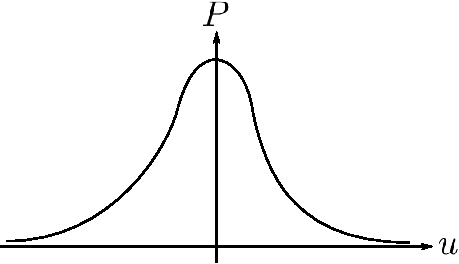
\includegraphics[width=2.7cm]{img/section2_fig20} &
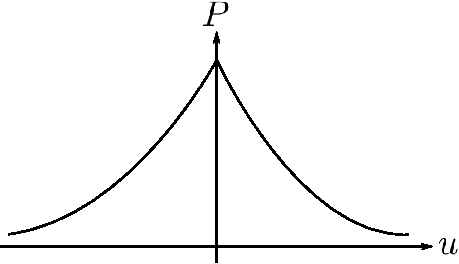
\includegraphics[width=2.7cm]{img/section2_fig21} & 
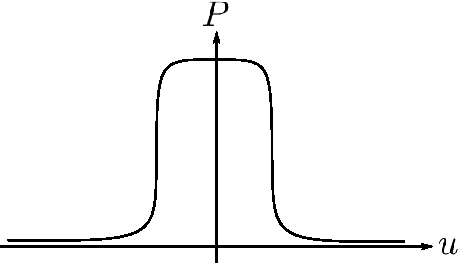
\includegraphics[width=2.7cm]{img/section2_fig22} \\ \\

& $\kurt(x) = 0$ & $\kurt(x) > 0$ & $\kurt(x) < 0$\\ \\

&
Gaussian PDF &
super-Gaussian PDF&
sub-Gaussian PDF\\
&bell shaped & peaky, long tails (``outliers'')& bulky, no ``outliers'' \\\\
e.g.&normal & Laplace & uniform
\end{tabular}\\[1cm]

\notesonly{This implies that we can use}
$|kurt(x)| > 0$ as a measure of nongaussianity 

\textbf{Caveat:}
\slidesonly{
sensitive to outliers
}
\end{frame}


\notesonly{
Kurtosis, just like other higher-order cumulants are sensitive to outliers, in that an outlier
 will register a much higher kurtosis value. This will be addressed later by FastICA.
}

\clearpage

\subsection{kurtosis-based ICA}

\begin{frame}{\subsecname}

\notesonly{
Two statistically independent sources with

$\langle s_i s_j \rangle = \delta_{ij} \quad \Leftrightarrow \quad \langle \vec s \, \vec s^\top \rangle = \vec I_N$ (any scaling can be attributed to $\vec A$)
}

\begin{equation*}
\widehat{s}_i \quad 
= \quad \vec{W}^\top \vec{x} \quad 
= \quad  \vec{W}^\top \vec{A} \cdot \vec{s} \quad 
=  \quad \vec{z}^\top \vec{s} \quad 
= \quad z_1 s_1 + z_2 s_2
\end{equation*}

\vspace{1mm}
We want the covariance of our reconstructions $\widehat{\vec s}$ to match that of the original sources $\vec s$.
\begin{equation*}
\langle \widehat{\vec s} \, \widehat{\vec s}^\top \rangle \eqexcl \langle \vec s \, \vec s^\top \rangle = \vec I_N
\end{equation*}
This implies,
\begin{align}
\var(\widehat{s}_i)
 \; &= \; \langle \big( z_1 s_1 + z_2 s_2 \big)^2 \rangle_{P_{\vec s}}\\
 \; &= \; \langle z_1^2 \, s_1^2 \rangle \;+\; 2 \, \langle z_1\, s_1\, z_2 \, s_2 \rangle \;+\; \langle z_2^2 \, s_2^2 \rangle \\
 \; &= \; z_1^2 \, \langle s_1^2 \rangle \;+\; 2 \, z_1\, z_2 \, \underbrace{\langle  s_1\,  s_2 \rangle}_{= 0} \;+\; z_2^2 \, \langle  s_2^2 \rangle \\
 \; &= \; z_1^2 \, \langle s_1^2 \rangle \;+\; z_2^2 \,\langle s_2^2 \rangle \\
 \; &= \; z_1^2 + z_2^2 \eqexcl 1
\end{align}

\end{frame}

\begin{frame}{\subsecname}

\slidesonly{
$$
\var(\widehat{s}_i)
 \; = \; z_1^2 + z_2^2 \eqexcl 1
 $$
}

Making the constraint of unit variance for $\widehat{s}_i$ is to match the variance assumed for the original sources $s_1$ and $s_2$. This implies that solutions for $\vec z$ are constrained to lie on a unit circle.
\vspace{1mm}
\begin{align*}
\kurt(\widehat{s})  \;\; &= \;\; \kurt(z_1 s_1 + z_2 s_2) \;\; \\ &= \;\; \kurt(z_1 s_1) + \kurt(z_2 s_2) \; = \; z_1^4 \kurt(s_1) + z_2^4 \kurt(s_2)
\end{align*}

\begin{block}{Kurtosis-based optimization problem}
\begin{equation*}
	\begin{array}{rllc}
	\left| \kurt(\widehat{s}) \right| & \eqexcl \max_{\vec{z}} 
	& \leftarrow & \substack{ 	\text{search for the direction} \\
					\text{with extreme kurtosis}} \\\\
	\var(\widehat{s}) = z_1^2 + z_2^2 & \eqexcl 1
	& \leftarrow & \substack{	\text{such that the data} \\
					\text{remains sphered}}
	\end{array} 
\end{equation*}
  \end{block}
\end{frame}

\begin{frame}
\slidesonly{
\begin{block}{Kurtosis-based optimization problem}
\begin{equation*}
	\begin{array}{rllc}
	\left| \kurt(\widehat{s}) \right| & \eqexcl \max_{\vec{z}} 
	& \leftarrow & \substack{ 	\text{search for the direction} \\
					\text{with extreme kurtosis}} \\\\
	\var(\widehat{s}) = z_1^2 + z_2^2 & \eqexcl 1
	& \leftarrow & \substack{	\text{such that the data} \\
					\text{remains sphered}}
	\end{array} 
\end{equation*}
  \end{block}
}


\begin{center}
$\hat{s} \,=\, \vec{z}^\top \vec{s} \,=\, \vec{w}^\top \underbrace{\vec{A} \, \vec{s}}_{\vec{x}} \,=\, \vec{b}^\top \underbrace{\tilde{\vec{A}} \, \vec{s}}_{\vec{u}}$ \hspace{4cm} $\kurt(s_i) \neq 0$
\end{center}

\question{What can we optimize kurtosis with?}

\pause
	\begin{enumerate}
		\item $\max_{\vec{z}} | \kurt{(\vec{z}^\top \vec{s})} | \; \; \;\quad s.t. \quad |\vec{z}| = 1$
		\item $\max_{\vec{w}} | \kurt{(\vec{w}^\top \vec{x})} | \quad s.t. \quad |\vec{A}^\top \vec{w}| = 1$
		\item $
        \max_{\vec{b}} | \kurt{(\vec{b}^\top \vec{u})} | \;\quad s.t. \quad 
        \underbrace{|\tilde{\vec{A}}^\top \vec{b}|
        }_{\substack{= |\vec{b}| \\ \text{ since } \tilde{\vec{A}} \\ \text{ is orthogonal}}} = 1
        $
	\end{enumerate}
\notesonly{
The different maximization approaches are equivalent. We opt for maximizing 
$| \kurt{(\vec{b}^\top \vec{u})} |$
because it is the only which we can obtain. The other terms either require access to the $\vec s$ or $\vec A$ which is not possible. 
Whitening $\vec x$ yields $\vec u$. We also do not know the orthogonal unmixing matrix $\widetilde{\vec A}$ but this
is not an issue because the orthogonality of $\widetilde{\vec A}$ lets the constraint 
reduce to only ensuring that $\vec b$ is kept at unit length.
}

\newpage

\end{frame}

\subsubsection{Kurtosis-based ICA: the gradient algorithm}

\begin{frame}{\subsubsecname}

\notesonly{
$| \kurt{(\vec{b}^\top \vec{u})} |$ can be maximized by moving $\vec b$ 
in the direction of the gradient until this becomes zero, whilst keeping the length of $\vec b$ equal to 1.
}

\begin{equation}
\label{eq:kurtgradient}
	\frac{\partial |\text{kurt}(\vec b^\top \vec u)|}{\partial \vec{b}} 
    =  4 \operatorname{sign} \left[ \kurt{(\vec{b}^\top \vec{u})} \right] \bigg( \langle \vec{u} (\vec{b}^\top \vec{u})^3 \rangle - 3 \vec{b} \, | \vec{b} |^2 \bigg) \eqexcl \vec{0}
\end{equation}
\begin{equation}
\label{eq:kurtgradientconstraint}
    \text{s.t. } \lVert{\vec{b}}\rVert^2 = 1
\end{equation}
\slidesonly{
\small{last term changes only length of $\vec{b} \leadsto$ can be removed due to constraint $\lVert{\vec{b}}\rVert^2 = 1$}
}
\notesonly{
We can omit the last term $3 \vec{b} \, | \vec{b} |^2$ as it only modifies the 
length of $\vec b$ which we want to keep equal to 1.
}
\normalsize
\begin{align}
\label{eq:kurtgradientsimple}
	\Delta \vec b &\propto 4 \operatorname{sign} \left[ \kurt{(\vec{b}^\top \vec{u})} \right] \langle \vec{u} (\vec{b}^\top \vec{u})^3 \rangle = \vec{0}\\
    \vec{b} &\leftarrow \vec{b} / \lVert{\vec{b}}\rVert^2
\end{align}

\notesonly{
where normalizing $\vec{b}$ ensures the constraint is satisfied. 
We can now describe an implementation of the Kurtosis-based gradient algorithm in its ``batch'' as well as its ``online'' form.
}

\end{frame}

\begin{frame}{\subsubsecname}

\begin{block}{I. batch learning:}
	Initialization: random vector $\vec{b}$ of unit length
	\begin{eqnarray*}
	\Delta \vec{b} &=& \varepsilon \operatorname{sign}\left[ \kurt{(\vec{b}^\top \vec{u})} \right] \langle \vec{u} (\vec{b}^\top \vec{u})^3 \rangle \\
	\vec{b} &\leftarrow& \vec{b} / |\vec{b}| \text{ (normalization to fulfill constraint |\vec{b}| = 1)}  
	\end{eqnarray*}
	
	\small
	ERM: replace expectations ($\kurt{(\cdot)}$ and $\langle \cdot \rangle$) by their respective empirical averages
	\normalsize
\end{block}
\end{frame}

\begin{frame}
\question{How to do online learning if the gradient requires computing expectations?}

\slidesonly{
\begin{align}
	\Delta \vec b \; &\propto \; 4 \operatorname{sign} \left[ \kurt{(\vec{b}^\top \vec{u})} \right] \langle \vec{u} (\vec{b}^\top \vec{u})^3 \rangle = \vec{0}\\
    \vec{b} \;&\leftarrow \;\vec{b} / |{\vec{b}}|
\end{align}

Recall:
    \begin{equation}
        \kurt (\vec{b}^\top \vec{u}) = \left\langle \left(\vec{b}^\top \vec{u}\right)^4 \right\rangle - 3 
    \end{equation}
}

\notesonly{
In order to apply the gradient algorithm in an online fashion as described by \eqref{eq:kurtgradientsimple}, we have to account for the fact that the kurtosis term inside our expression for the gradient involves an expectation operator which cannot be omitted (cf. \eqref{eq:kurt} for how kurtosis is defined). We therefore resort to estimating the kurtosis from a moving average $\gamma$ which starts at zero and is updated at each iteration using:
}
\slidesonly{
Estimate kurtosis via moving average:
}
\begin{equation}
\label{eq:gammaupdate}
\Delta \gamma = \eta \left[ (\vec{b}^\top \vec{u})^4 -3 - \gamma \right]
\end{equation}
\slidesonly{
where $\gamma$ is initialized with 0.
}
\end{frame}
\begin{frame}

\begin{block}{II. online learning:}
	Initialization: random vector $\vec{b}$ of unit length, $\gamma = 0$ \\\vspace{0.2cm}
	choose a data point $\vec{u}$
	\vspace{-0.2cm}
	\begin{eqnarray*}
	\Delta \vec{b} &=& \varepsilon \operatorname{sign} (\gamma) \; \vec{u} (\vec{b}^\top \vec{u})^3 \hspace{0.25cm} \quad\;\, \substack{\text{\hspace{0.6mm}(weight update per data point)}} \\
	\Delta \gamma &=& \eta \left[ (\vec{b}^\top \vec{u})^4 -3 - \gamma \right] \hspace{0.25cm} \quad \substack{\text{(running average of the kurtosis with learning rate } \eta )} \\
	\vec{b} &\leftarrow& \vec{b} / |\vec{b}|
	\end{eqnarray*}
\end{block}
\end{frame}

\begin{frame}
\frametitle{The gradient algorithm - advantages and disadvantages}
\textbf{Advantage(s)}:
\pause
\begin{itemize}
\item online learning to adapt to non-stationary data
\end{itemize}
\textbf{Disadvantage(s)}:
\pause
\begin{itemize}
\item dependent on good choice of learning rate and its schedule (i.e. decay over time)
\end{itemize}

\slidesonly{
\vspace{2cm}
$\leadsto$ fixed-point iteration alternative
}
\notesonly{
A fixed-point iteration algorithm provides an alternative to make the learning faster and more reliable without the need for deciding on a learning rate and its sequence.
}
\end{frame}

\subsubsection{Fixed-point iteration}

\begin{frame}{\subsubsecname}

\begin{itemize}
\item A fixed point: $x=g(x)=g(g(\ldots g(x)\ldots))$\\

Example:
\begin{align}
    g(x) &= x^{2} - 3x + 4\\
    g(2) &= 2^{2} - 3\cdot 2 + 4 = 4 - 6 + 4 = 2
\end{align}

\item Fixed point iteration:
\begin{equation}
x^{(t+1)} = g(x^{(t)}), t=0,1,2,\ldots
\end{equation}
\end{itemize}

\begin{center}
    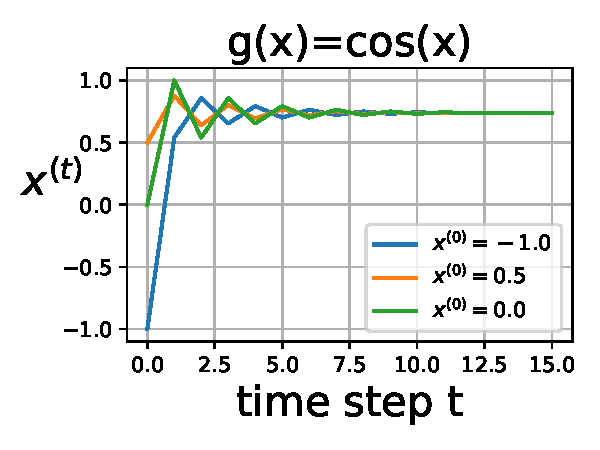
\includegraphics[height=3.5cm]{img/fixed_point_iter_cos} 
    \mode<article>{
    \captionof{figure}{
    Fixed point iteration example
    }
    \label{fig:fixedpointcos}
    } 
\end{center}

\end{frame}

\begin{frame}

\notesonly{
A stable point of the gradient algorithm is when the gradient points in the same direction of $\vec b$ which leads to not having to update $\vec b$ (i.e. change its direction) any further. This is also the case when the gradient algorithm has converged. We won't go into a rigorous justification of this \footnote{If interested, see Hyv{\"a}rinen Ch. 8.2.3 and Ex 3.9 from the same book.}

Below is a realization of this faster fixed-point iteration alternative of the Kurtosis-based ICA (The kurtosis-based fastICA should not be confused with the fastICA algorithm we will discussed later.)
}

\begin{block}{III. fixed-point algorithm (\textbf{kurtosis-based} fastICA)}
	fixed point condition of gradient descent: $\vec{b} \propto \Delta \vec{b}$ \\
	$\leadsto \vec{b} \propto \langle \vec{u} (\vec{b}^\top \vec{u})^3 \rangle - 3 |\vec{b}|^2 \vec{b}$ \\\vspace{0.2cm}
	exploiting normalization $(|\vec{b}|^2 = 1)$ we have:
	\vspace{-0.3cm}
	\begin{eqnarray*}
		\vec{b} &\leftarrow& \langle \vec{u} (\vec{b}^\top \vec{u})^3 \rangle - 3 \vec{b} \\
		\vec{b} &\leftarrow& \vec{b} / |\vec{b}|
	\end{eqnarray*} \\
	kurtosis-based fastICA-algorithm for whitened data $\vec{u}^{(\alpha)},\, \alpha = 1, \dots, p$: \\[5pt]
	initialization: random vector $\vec{b}$ of unit length, then iterate:\\
	\vspace{-0.6cm}
	\begin{eqnarray*}
	\vec{b} &\leftarrow& \frac{1}{p} \sum_{\alpha=1}^{p} \vec{u}^{(\alpha)} (\vec{b}^\top \vec{u}^{(\alpha)})^3 - 3 \vec{b} \\
	\vec{b} &\leftarrow& \vec{b} / |\vec{b}|
	\end{eqnarray*} \\
\end{block}
\end{frame}

%\slidesonly{
%\begin{frame}
%\frametitle{Summary so far:}
%\begin{enumerate}
%\item \textcolor{gray}{
%Initial ICA Problem: $\vec x = \vec A\, \vec s$
%}
%\item \textcolor{gray}{
%New ICA Problem: $\vec u = \widetilde{\vec A}\, \vec s$,\\
%where $\vec u = \vec D^{-\frac{1}{2}} \vec U^\top \vec x$ and $\vec \Sigma_u = \vec I_N$.
%}
%\item \textcolor{gray}{
%$\vec u$ is the \emph{whitened} version of $\vec x$.
%}
%\item \textcolor{gray}{
%$\vec D$ and $\vec U$ can be obtained via PCA on $\vec x$.
%}
%\item \textcolor{gray}{
%Applying ICA on whitened data reduced the number of free parameters.
%}
%\item \textcolor{gray}{
%PCA simplifies the ICA problem.
%}
%\item Ambiguities in ICA
%\item Why are Gaussians bad for ICA?
%\item ICA by maximizing nongaussianity
%\item Kurtosis-based ICA

%\end{enumerate}



%\end{frame}
%}
\notesonly{
Next, we will look for an alternative that mitigates the sensitivity to outliers which kurtosis-based ICA is prone to.
}

\begin{frame}

\slidesonly{

\textbf{Next: Can we do better than kurtosis-based ICA?}

\vspace{5mm}

\pause 
}

Kurtosis is easy to compute but can be \emph{sensitive to outliers}. 
This is a usual problem with higher-order statistics. 
\begin{block}{Example}
\begin{itemize}
  \item Sample of 1000 values from a distribution with mean = 0 and std=1
  \item One observation with $x=10$ after sphering:
  \itl contribution to kurtosis: $ \geq 10^4/1000 -3 = 7$
\end{itemize}
\end{block}

\pause

\slidesonly{
$\Rightarrow\;\;$ a more robust measure for nongaussianity\\
}
\notesonly{We therefore turn to an alternate measure for nongaussianity, namely }\emph{negentropy} \notesonly{for brevity }(not the same as negative entropy $-H(\cdot)$).\\

%\svspace{5mm}
\notesonly{
Negentropy of the reconstructed source $\widehat{\vec s}$ measures the difference between the differential entropy of $\widehat{\vec s}$ and the differential entropy of a Gaussian distribution with the same variance as $\widehat{\vec s}$.
}

\end{frame}
